%! root=../main.tex
\begin{figure}
    \centering
    \resizebox{.9\linewidth}{!}{
    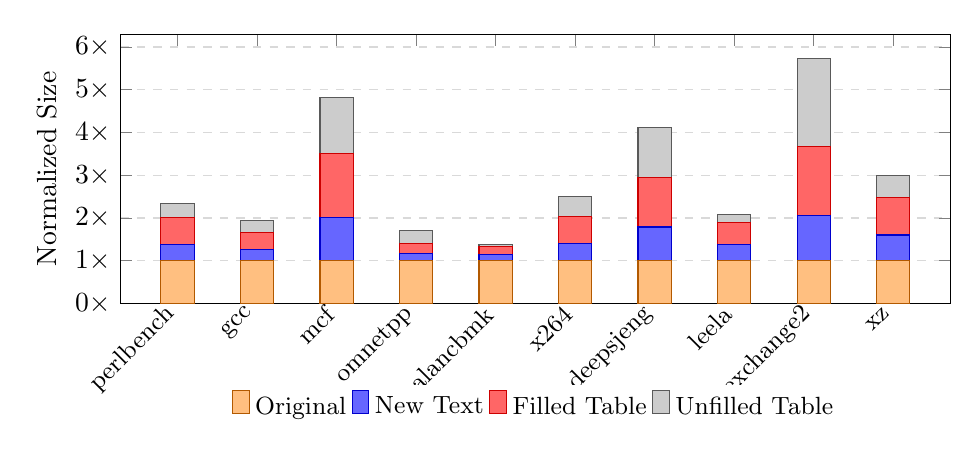
\begin{tikzpicture}
        \begin{axis}[
            ybar stacked,
            bar width=12pt,
            enlarge x limits=0.08,
            ylabel={Normalized Size},
            ymin=0,
            width=\columnwidth,
            height=5cm,
            yticklabel=$\pgfmathprintnumber{\tick}\times$,
            symbolic x coords={
                perlbench,
                gcc,
                mcf,
                omnetpp,
                xalancbmk,
                x264,
                deepsjeng,
                leela,
                exchange2,
                xz,
            },
            xtick=data,
            x tick label style={rotate=45, anchor=east, font=\small},
            ytick distance=1,
            legend style={
                at={(0.5,-0.3)},
                anchor=north,
                legend columns=-1,
                draw=none,
                font=\small
            },
            ymajorgrids=true,
            major grid style={dashed, gray!30},
        ]

        \addplot+[ybar, fill=orange!50, draw=orange!70!black] coordinates {
            (perlbench, 1)
            (gcc, 1)
            (mcf, 1)
            (omnetpp, 1)
            (xalancbmk, 1)
            (x264, 1)
            (deepsjeng, 1)
            (leela, 1)
            (exchange2, 1)
            (xz, 1)
        };
        \addplot+[ybar, fill=blue!60, draw=blue!80!black] coordinates {
            (perlbench, 0.3859)
            (gcc, 0.2545)
            (mcf, 1.0217)
            (omnetpp, 0.1686)
            (xalancbmk, 0.1391)
            (x264, 0.4007)
            (deepsjeng, 0.7891)
            (leela, 0.3768)
            (exchange2, 1.0673)
            (xz, 0.6035)
        };

        \addplot+[ybar, fill=red!60, draw=red!80!black] coordinates {
            (perlbench, 0.6169)
            (gcc, 0.4040)
            (mcf, 1.4813)
            (omnetpp, 0.2281)
            (xalancbmk, 0.1864)
            (x264, 0.6400)
            (deepsjeng, 1.1660)
            (leela, 0.5262)
            (exchange2, 1.6062)
            (xz, 0.8843)
        };

        \addplot+[ybar, fill=gray!40, draw=gray!70!black] coordinates {
            (perlbench, 0.3261)
            (gcc, 0.2842)
            (mcf, 1.3159)
            (omnetpp, 0.3195)
            (xalancbmk, 0.0530)
            (x264, 0.4600)
            (deepsjeng, 1.1660)
            (leela, 0.1753)
            (exchange2, 2.0490)
            (xz, 0.5139)
        };

        \legend{Original, New Text, Filled Table, Unfilled Table}
        \end{axis}
    \end{tikzpicture}}
    \caption{Space overhead for each benchmark showing the contributions of the new text and table segments. Unfilled table entries can be decreased with a better hash function.\ixb{Notice that 2 benchmarks with little unfilled data have really high overheads (leela~34\%, xalancbkm~20\%)}}
    \label{fig:spec2017_size}
\end{figure}
